%%%%%%%%%%%%%%%%%%%%%%%%%%%%%%%%%%%%%%%%%%%%%%%%%%%%%%%%%%%%%%%%%%%%%%%
% Electronic Supplementary Information (ESI) for the ChEmbed manuscript.
%
% Scope: expands the two diagnostics reported in Section 5.3 of the paper,
% "Impact of Task and Domain Adaptation".
%
% RSC provides no ESI template. The running header and copyright line are
% added by RSC production after acceptance and are not included here.
% Section and figure numbers carry an "S" prefix.
%
% >>> BEFORE SUBMISSION <<<
%   Uncomment the \dag ESI footnote in paper.tex and add \dag to the title.
%
% Build: pdflatex esi ; bibtex esi ; pdflatex esi ; pdflatex esi
%%%%%%%%%%%%%%%%%%%%%%%%%%%%%%%%%%%%%%%%%%%%%%%%%%%%%%%%%%%%%%%%%%%%%%%

\documentclass[11pt]{article}

\usepackage[a4paper, margin=2.2cm]{geometry}
\usepackage[T1]{fontenc}
\usepackage{mathptmx}
\usepackage{amsmath,amssymb}
\usepackage{graphicx}
\usepackage{float}
\usepackage{setspace}
\usepackage[format=plain,justification=justified,singlelinecheck=false,labelfont=bf,labelsep=period,font=small]{caption}
\usepackage[super,sort&compress,comma]{natbib}
\usepackage[colorlinks=true,allcolors=blue,
            pdftitle={Supplementary Information for ChEmbed: Enhancing Chemical Literature Search Through Domain-Specific Text Embeddings},
            pdfauthor={Ali Shiraee Kasmaee, Mohammad Khodadad, Mahdi Astaraki, Mohammad Arshi Saloot, Nicholas Sherck, Hamidreza Mahyar, Soheila Samiee}]{hyperref}

\renewcommand{\thesection}{S\arabic{section}}
\renewcommand{\thefigure}{S\arabic{figure}}
\renewcommand{\theequation}{S\arabic{equation}}
% Slightly relaxed leading and visible, restrained separation between paragraphs.
\setstretch{1.035}
\setlength{\parindent}{0pt}
\setlength{\parskip}{7pt plus 1.5pt minus 1pt}
\setlength{\bibsep}{3pt}

\newcommand{\CEv}{ChEmbed\textsubscript{vanilla}}
\newcommand{\CEp}{ChEmbed\textsubscript{progressive}}

\title{%
  \large\textbf{Supplementary Information for:}\\[6pt]
  \Large\textbf{ChEmbed: Enhancing Chemical Literature Search Through\\Domain-Specific Text Embeddings}%
}
\author{%
  \normalsize Ali Shiraee Kasmaee, Mohammad Khodadad, Mahdi Astaraki, Mohammad Arshi Saloot,\\
  \normalsize Nicholas Sherck, Hamidreza Mahyar and Soheila Samiee
}
\date{}

\begin{document}

\maketitle
\vspace{-1.5em}

Section 5.3 of the main text presents two related diagnostic analyses. The
first asks whether chemistry literature and chemistry-related encyclopedic
text are already distinguishable in the unmodified base-model space; the
second examines how fine-tuning changes the representations of the same
passages. This supplement describes the design and evidence supporting both
parts of that argument.

\section{Sampling and encoding}
\label{sec:esi-sampling}

We analyzed passages from the three retrieval benchmarks used in the main
paper: ChemRxiv Retrieval, ChemNQ Retrieval and ChemHotpotQA Retrieval. To make
the sampled passages independent at the source-document level, we grouped
ChemRxiv passages by preprint and grouped ChemNQ and ChemHotpotQA passages by
their source encyclopedia page, then retained one passage from each group. The
primary comparison contained 800 ChemRxiv paragraphs and an equally sized
encyclopedic sample composed of 400 ChemNQ and 400 ChemHotpotQA passages;
sampling used seed 1337.

All three models, the \texttt{nomic-embed-text-v1} base encoder and the two
adapted variants, received the same 1{,}600 passages after identical text
preprocessing. Each input began with the model's document-search prefix
\texttt{search\_document:}. The encyclopedic benchmark records store the
source-page title separately from the passage body, so this existing title
field was placed before the passage text, as in the retrieval evaluation.
ChemRxiv records have no separate title field and were therefore encoded using
the paragraph text alone. The resulting
768-dimensional embeddings were L2-normalized, and inference was performed on
CPU in single precision. We use \CEv{} as the primary adapted model because it
isolates the effect of fine-tuning from the tokenizer augmentation discussed in
Section 5.2 of the main text, while \CEp{} provides a complementary sensitivity
comparison.

\section{Separation before fine-tuning}
\label{sec:esi-separation}

The three corpora all concern chemistry, but they differ in genre, provenance,
formatting and possibly in their topic distributions. We therefore
asked a narrower question: before any ChEmbed fine-tuning, does the
base model represent the literature and encyclopedic samples as measurably
different populations?

To answer this question, we reduced the base-model embeddings to 64 principal
components, standardized them and fitted logistic regression under stratified
five-fold cross-validation. Dimensionality reduction and scaling were repeated
inside each training fold, preventing information from the held-out passages
from entering the classifier. The resulting out-of-fold accuracy was 95.6\%
(95\% bootstrap interval 94.6--96.6\%); because the two classes were balanced,
uninformative predictions would be correct only about half of the time. To test
whether the observed accuracy could arise by chance, we repeated the analysis
999 times after randomly shuffling the literature and encyclopedic labels.
None of these shuffled analyses reached the observed accuracy, giving
$p=0.001$. Changing the projection size or cross-validation seed produced
accuracies between 94.9\% and 96.1\%. This use of classification as a two-sample
test follows the general framework of Lopez-Paz and Oquab
\citep{lopezpaz2017revisiting}.

Passage length contributed to the distinction without accounting for most of
it. A probe based only on word and character counts reached 76.1\% accuracy,
reflecting the greater average length of the preprint paragraphs. We therefore
matched literature and encyclopedic passages within ten passage-length bands,
leaving 766 documents with comparable length distributions. On this matched
subset, a classifier using only word and character counts performed at chance
(47.1\%), while the embedding-based classifier remained accurate (93.6\%). A
local analysis led to the same conclusion: among the ten nearest neighbors of
each passage, 86.4\% came from the same corpus class, rather than the
approximately even mixture expected if the classes were interchangeable
\citep{schilling1986multivariate}.

Figure~\ref{fig:esi-separation} shows this result directly. PCA selected the
two directions that capture the most variation among the passage embeddings
without reference to the corpus labels. Although these two directions contain
only a small part of the total variance, they already reveal substantial
separation.

Together, the classifier, length-matched control and neighborhood analysis show
that the two corpora differ in their base-model representations. They do not
identify the source of that difference, which may combine genre, topic,
formatting and collection provenance.

\begin{figure}[H]
\centering
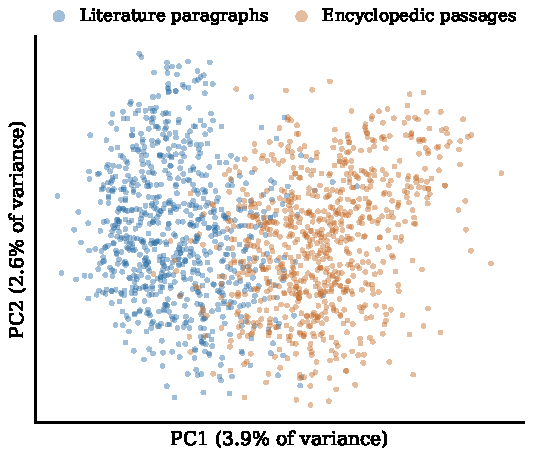
\includegraphics[width=0.55\linewidth]{figures/esi_separation}
\caption{Literature and encyclopedic passages in the base model, projected onto
their first two principal components. PCA calculated the projection from the
embeddings alone, and the corpus colors were added afterward. Although the two
components contain only a small share of the total variance, the classes
already occupy substantially different regions.}
\label{fig:esi-separation}
\end{figure}

\section{Changes from fine-tuning}
\label{sec:esi-change}

We next encoded the same passages with the adapted models and compared the
resulting spaces with the base representation. The clearest change concerned
angular dispersion. For ChemRxiv, mean pairwise cosine similarity fell from
0.570 in the base model to 0.030 under \CEv{}, whereas the encyclopedic pool
changed from 0.517 to 0.163. Mean similarity therefore decreased by 0.540 for
ChemRxiv and by 0.354 for the encyclopedic pool: the ChemRxiv decrease was
0.187 greater (95\% bootstrap interval 0.180--0.195). \CEp{} produced the same
qualitative pattern. Fine-tuning therefore dispersed both corpora, more
strongly for the literature passages (Figure~\ref{fig:esi-dispersion}). This
measure describes the concentration of the embedding space; on its own, it does
not show that individual passages became easier to retrieve
\citep{ethayarajh2019contextual}.

The change in local structure was more modest and depended on the scale of the
neighborhood. For each passage, we identified its ten closest passages before
fine-tuning and then counted how many remained among its ten closest passages
after fine-tuning. Under \CEv{}, the average overlap was 35.4\% for ChemRxiv
and 42.7\% for the encyclopedic passages, indicating somewhat greater local
change for ChemRxiv. This difference disappeared when the neighborhood was
expanded from ten to fifty passages (44.0\% against 43.9\%), while the
corresponding \CEp{} comparison reversed direction at the wider scale
(49.7\% against 46.0\%). Linear centered kernel alignment
agreed with the ten-neighbor result \citep{kornblith2019similarity}, but we did
not use it for inference because ordinary bootstrap resampling was strongly
biased at this sample size. These
results support a graded, scale-dependent specialization rather than a
wholesale reorganization confined to chemistry literature.

\begin{figure}[H]
\centering
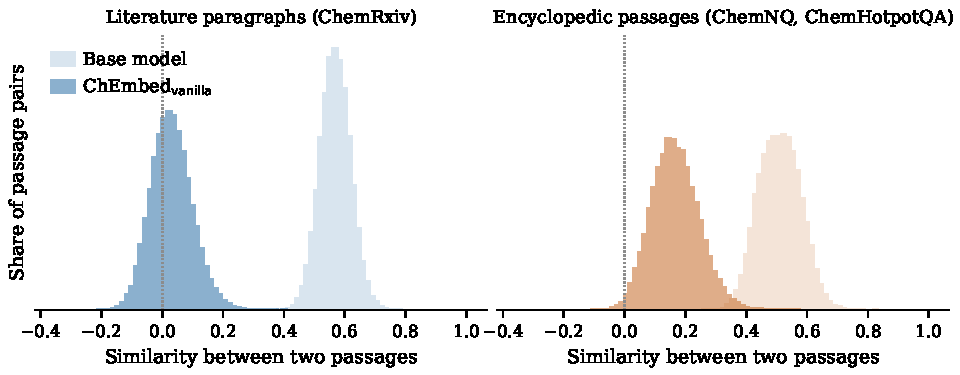
\includegraphics[width=\linewidth]{figures/esi_dispersion}
\caption{Distributions of pairwise cosine similarity before and after
fine-tuning with \CEv{}. Mean similarity falls from 0.570 to 0.030 for the
ChemRxiv literature passages and from 0.517 to 0.163 for the balanced
encyclopedic pool.}
\label{fig:esi-dispersion}
\end{figure}

\section{Limitations}
\label{sec:esi-limits}

These analyses are observational: they establish that the sampled corpora are
distinguishable in the base-model space and that fine-tuning changes their
representations to different degrees, but they neither isolate the corpus
property responsible for the separation nor demonstrate that the geometric
changes caused the retrieval results. The geometry analysis also relies on one
sampling seed, and the two encyclopedic retrieval tasks contain very few test
queries. Their associated score differences should therefore be interpreted as
indicative rather than conclusive.

\bibliography{references}
\bibliographystyle{rsc}

\end{document}
